\documentclass[12pt,a4paper]{article}

% Paquetes básicos
\usepackage[utf8]{inputenc}
\usepackage[T1]{fontenc}
\usepackage[english]{babel}
\usepackage{amsmath, amssymb}
\usepackage{siunitx} 
\usepackage{graphicx}
\usepackage{float}
\usepackage{geometry}
\usepackage{xcolor}
\geometry{margin=2.5cm}
\usepackage{hyperref}
\usepackage{caption}
\usepackage{subcaption}
\usepackage{setspace}
\usepackage{multirow}
\usepackage{minted}  
\usepackage{gensymb} 
\usepackage[backend=biber, style=ieee]{biblatex}
\usepackage[american, straightvoltages]{circuitikz}
\usepackage{csquotes}
\usepackage{indentfirst}
\addbibresource{references.bib}

\graphicspath{{Figures/}}
\onehalfspacing
\hypersetup{
    colorlinks  = true,
    linkcolor   = blue,    
    citecolor   = blue,
    urlcolor    = blue,
    filecolor   = blue
}

\begin{document}       
\renewcommand{\figureautorefname}{Fig.}
\renewcommand{\tableautorefname}{Tab.}
\renewcommand{\equationautorefname}{Eq.}


% Carátula personalizada
\begin{titlepage}
    \centering
    
\includegraphics[width=0.7\textwidth]{Fulgor Logo.png}\\[1.5cm]

    {\Large \textbf{FUNDACIÓN FULGOR} \\[0.5cm]}
    {\Large CMOS Course} \\[0.5cm]

    \rule{\textwidth}{0.5pt} \\[0.5cm]
    {\Large \textbf{Homework N°2} \\[0.3cm]}
    \rule{\textwidth}{0.5pt} \\[1cm]
    
\begin{tabular}{l l}
    \textbf{Professors:} & Michel Saenz.\\
                         & Santiago Castro.\\
    \\
    \textbf{Student:}    & Monja, Ernesto Joaquín (43.873.728)\\
\end{tabular} \\[5cm]

{\centering Year 2026 \par}

\end{titlepage}



% Índice
\tableofcontents
\newpage



\section{Introduction}
This report presents the small-signal alternating current (\textit{AC}) analysis for the assigned \textit{CMOS} amplifier circuit shown in \autoref{fig:fig_1}.
\begin{figure}[H]
    \centering
    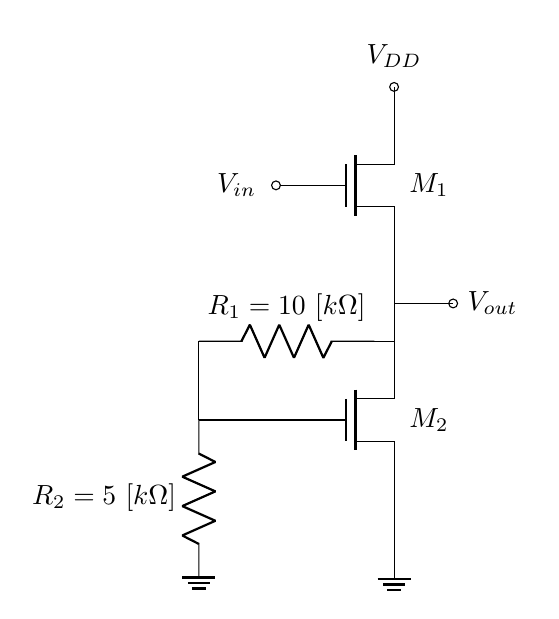
\begin{tikzpicture}[transform shape]
	% Paths, nodes and wires:
	\node[nmos](N1) at (0, 1.48){} node[anchor=west] at (N1.text){$M_{1}$};
	\node[nmos](N2) at (0, -1.5){} node[anchor=west] at (N2.text){$M_{2}$};
	\draw (-1.5, 1.48) -- (-0.98, 1.48);
	\draw (0, 0.71) -- (0, -0.75);
	\draw (-2.48, -3.5) to[american resistor, l={$R_{2} = 5 \ [k\Omega]$}] (-2.48, -1.5);
	\draw (-0, -2.27) -| (0, -2.29) -- (-0, -3.52);
	\draw (-2.48, -0.5) to[american resistor, l={$R_{1} = 10 \ [k\Omega]$}] (-0.25, -0.5);
	\draw (-2.48, -0.5) -| (-2.48, -1.5);
	\node[tlground] at (-2.48, -3.5){};
	\node[tlground] at (-0, -3.52){};
	\node[shape=rectangle, minimum width=0.965cm, minimum height=0.465cm](N3) at (-2, 1.48){} node[anchor=center] at (N3.text){$V_{in}$};
	\node[ocirc] at (-1.5, 1.48){};
	\node[ocirc] at (-0, 2.73){};
	\node[ocirc] at (0.75, -0.02){};
	\draw (-0, 2.73) -| (0, 2.25);
	\draw (0.75, -0.02) -- (-0, -0.02);
	\node[shape=rectangle, minimum width=0.965cm, minimum height=0.465cm](N4) at (1.25, -0.02){} node[anchor=center] at (N4.text){$V_{out}$};
	\node[shape=rectangle, minimum width=0.715cm, minimum height=0.715cm](N5) at (0, 3.125){} node[anchor=center] at (N5.text){$V_{DD}$};
	\draw (-0.98, -1.5) -| (-2.48, -1.5);
	\draw (-0.25, -0.5) -- (0, -0.5);
\end{tikzpicture}
    \caption{Circuit proposed to analyze.} 
    \label{fig:fig_1}
\end{figure}

The circuit topology in \autoref{fig:fig_1} is identified as a \textit{Common-Drain} amplifier, also known as a \textit{Source Follower} \cite[p. 331]{b1}. In this configuration, the input signal is applied to the gate of transistor $M_{1}$, and the output is taken at its source. The transistor $M_{2}$ acts as an active load; however, unlike a standard source follower with a fixed bias, its gate is tied to a local negative feedback loop formed by the voltage divider $R_{1}$ and $R_{2}$. The objective of this report is to derive the complete small-signal voltage gain $A_{v}$ considering channel-length modulation effects (this is assuming that $r_{o} = 5 \ [k\Omega]$ for both transisors) and lastly we´ll use the following trans-conductance values for $M_{1}$ and $M_{2}$:
\begin{itemize}
    \item $g_{m1} = 1 \ [mS]$
    \item $g_{m2} = 3 \ [mS]$
\end{itemize}



\section{Development and Small-Signal Analysis}
To accurately model the circuit in the small-signal domain, the \textit{DC} supply $V_{DD}$ is considered as an \textit{AC} ground. Transistors $M_{1}$ and $M_{2}$ are replaced by their respective small-signal equivalents, including their output resistances $r_{O1}$ and $r_{O2}$ to provide a realistic estimation of the circuit's behavior. Therefore, the small signal circuit representation of \autoref{fig:fig_1}, is shown in \autoref{fig:fig_2}
\begin{figure}[H]
    \centering
    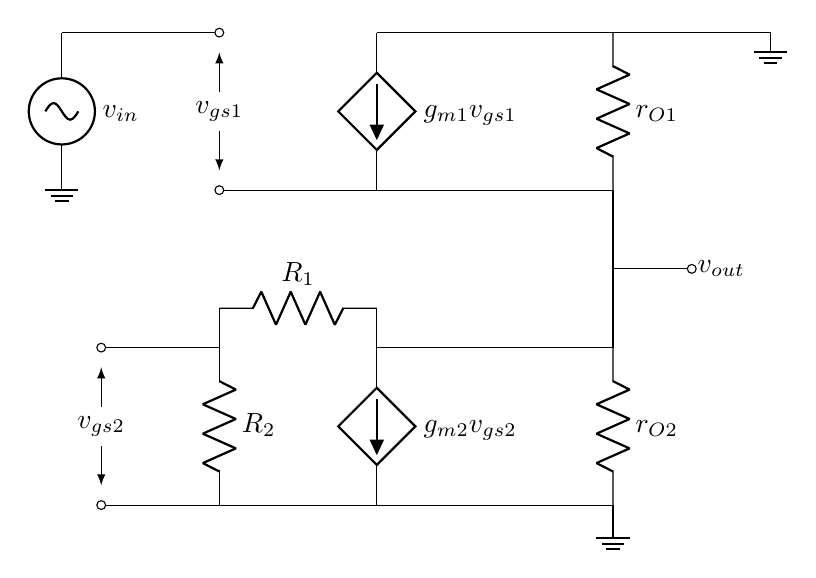
\begin{tikzpicture}[transform shape]
	% Paths, nodes and wires:
	\draw (3, 3) to[american resistor, l={$r_{O1}$}] (3, 1);
	\draw (-0, 3) to[american controlled current source, l={$g_{m1}v_{gs1}$}] (-0, 1);
	\draw (-0, 3) -- (3, 3);
	\draw (-4, 3) to[sinusoidal voltage source, l={$v_{in}$}] (-4, 1);
	\draw (-4, 3) -- (-2, 3);
	\draw (-2, 1) -- (3, 1);
	\draw (3, 3) -- (5, 3) -| (5, 2.75);
	\node[tlground] at (5, 2.75){};
	\draw (3, 1) -- (3, -0) -- (4, -0) -- (3, -0) -| (3, -1) -- (1, -1);
	\draw (3, -1) to[american resistor, l={$r_{O2}$}] (3, -3);
	\draw (-2, -0.5) to[american resistor, l={$R_{1}$}] (-0, -0.5);
	\draw (-2, -1) to[american resistor, l={$R_{2}$}] (-2, -3);
	\draw (-2, -0.5) -| (-2, -1);
	\draw (-0, -1) -- (1, -1);
	\draw (-2, -3) -- (3, -3);
	\draw (-0, -1) to[american controlled current source, l={$g_{m2}v_{gs2}$}] (-0, -3);
	\node[ground] at (3, -3){};
	\node[shape=rectangle, minimum width=0.715cm, minimum height=0.465cm](N1) at (4.375, -0){} node[anchor=center] at (N1.text){$v_{out}$};
	\node[shape=rectangle, minimum width=0.715cm, minimum height=0.465cm](N2) at (-2, 2){} node[anchor=center] at (N2.text){$v_{gs1}$};
	\draw (-0, -0.5) -| (-0, -1);
	\draw (-2, -1) -- (-3.5, -1);
	\draw (-2, -3) |- (-3.5, -3);
	\node[shape=rectangle, minimum width=0.715cm, minimum height=0.465cm](N3) at (-3.5, -2){} node[anchor=center] at (N3.text){$v_{gs2}$};
	\draw (-3.5, -1) to[open] (-3.5, -3);
	\node[ocirc] at (-2, 3){};
	\node[ocirc] at (-3.5, -1){};
	\node[ocirc] at (-3.5, -3){};
	\node[ocirc] at (4, -0){};
	\draw[-latex] (-2, 2.25) -- (-2, 2.75);
	\draw[-latex] (-2, 1.75) -- (-2, 1.25);
	\draw[-latex] (-3.5, -1.75) -- (-3.5, -1.25);
	\draw[-latex] (-3.5, -2.25) -- (-3.5, -2.75);
	\node[tlground] at (-4, 1){};
	\node[ocirc] at (-2, 1){};
\end{tikzpicture}
    \caption{Complete small-signal equivalent circuit configuration featuring finite output resistances and local negative feedback network.}
    \label{fig:fig_2}
\end{figure}

Given the circuit shown in \autoref{fig:fig_2}, we can start doing the analysis of the small signal in order to calculate the voltage gain of it. We can do this process step by step in the following subsections.


\subsection{Defining the Control Voltages}
First, we must define the gate-to-source voltages ($v_{gs}$) that control the dependent current sources of transistors $M_{1}$ and $M_{2}$. For the input transistor $M_{1}$, the input voltage $V_{in}$ is applied at the gate, and the output $v_{out}$ is located at the source. Thus, the control voltage is:
\begin{equation}
    v_{gs1} = v_{in} - v_{out}
    \label{eq_1}
\end{equation}

For the active load transistor $M_{2}$, the gate voltage is defined by the voltage divider formed by $R_1$ and $R_2$, which is fed by the output node $v_{out}$. Therefore:
\begin{equation}
    v_{gs2} = v_{out} \left(\frac{R_{2}}{R_{1} + R_{2}}\right)
    \label{eq_2}
\end{equation}


\subsection{Applying Kirchhoff's Current Law}
We apply Kirchhoff's Current Law at the $v_{out}$ node, stating that the sum of the currents entering the node equals the sum of the currents leaving the node towards the AC ground. Therefore, the current entering the node from the dependent source of $M_1$ is:
\begin{equation}
    i_{in} = g_{m1}v_{gs1} = g_{m1}(v_{in} - v_{out})
    \label{eq_3}
\end{equation}

The currents leaving the node are distributed through four parallel paths: the output resistance of $M_{1}$ ($r_{O1}$), the output resistance of $M_{2}$ ($r_{O2}$), the resistive feedback branch ($R_{1} + R_{2}$), and the dependent current source of $M_{2}$. The total leaving current is:
\begin{equation}
    i_{out} = \frac{v_{out}}{r_{O1}} + \frac{v_{out}}{r_{O2}} + \frac{v_{out}}{R_{1} + R_{2}} + g_{m2}v_{gs2}
    \label{eq_4}
\end{equation}


\subsection{Analytical Expression for the Voltage Gain}
Due to the fact that the entering and leaving currents have to be the same, this is the mathematical equivalent to equating \autoref{eq_3} and \autoref{eq_4} and thus:
\begin{equation}
    g_{m1}(v_{in} - v_{out}) = \frac{v_{out}}{r_{O1}} + \frac{v_{out}}{r_{O2}} + \frac{v_{out}}{R_{1} + R_{2}} + g_{m2}v_{gs2}
    \label{eq_5}
\end{equation}

Substituting the expression for $v_{gs2}$ found in \autoref{eq_2}, we have:
\begin{equation}
    g_{m1}(v_{in} - v_{out}) = \frac{v_{out}}{r_{O1}} + \frac{v_{out}}{r_{O2}} + \frac{v_{out}}{R_{1} + R_{2}} + g_{m2} \left(v_{out}\frac{R_{2}}{R_{1} + R_{2}}\right)
    \label{eq_6}
\end{equation}

By distributing the $g_{m1}$ term in the left side of the \autoref{eq_6} and grouping all the $v_{out}$ terms on the right side of the equation, we obtain:
\begin{equation}
    g_{m1}v_{in} = v_{out} \left( g_{m1} + \frac{1}{r_{O1}} + \frac{1}{r_{O2}} + \frac{1}{R_{1} + R_{2}} + g_{m2} \frac{R_{2}}{R_{1} + R_{2}} \right)
    \label{eq_7}
\end{equation}

Finally, solving for the voltage gain $A_{v} = v_{out}/v_{in}$ yields the analytical expression:
\begin{equation}
    A_{v} = \frac{g_{m1}}{g_{m1} + \frac{1}{r_{O1}} + \frac{1}{r_{O2}} + \frac{1}{R_{1} + R_{2}} + g_{m2} \frac{R_{2}}{R_{1} + R_{2}}}
    \label{eq_8}
\end{equation}


\subsection{Numerical Calculation}
Using the given design parameters and the assumed output resistances ($r_{O1} = r_{O2} = 5 \ [k\Omega]$), we can compute the final value of the voltage gain obtained in \autoref{eq_8}:
\begin{equation}
    A_{v} = \frac{1 \ [mS]}{1 \ [mS] + \frac{1}{5 \ [k\Omega]} + \frac{1}{5 \ [k\Omega]} + \frac{1}{10 \ [k\Omega] + 5 \ [k\Omega]} + 3 \ [mS] \frac{5 \ [k\Omega]}{10 \ [k\Omega] + 5 \ [k\Omega]}} \approx 0.4054 \left[ \frac{V}{V} \right]
    \label{eq_9}
\end{equation}



\section{Conclusion}
The small-signal analysis yields a numerical voltage gain of approximately $0.4 \ \left[\frac{V}{V}\right]$. This sub-unity gain is theoretically consistent with a \textit{Source Follower} topology \cite[p. 332]{b1}. The result demonstrates that the inclusion of non-idealistic (finite) output impedances ($r_{O1}$ and $r_{O2}$), along with the active participation of $M_{2}$ through the local negative feedback network, significantly loads the output node, attenuating the ideal unity gain down to approximately $40.5 \ [\%]$.

\newpage
\printbibliography[heading=bibintoc, title={4 \, \, Bibliography}]
\end{document}